\section*{Assignment 07: Inequality and Responsibility}
\addcontentsline{toc}{section}{Assignment 07: Inequality and Responsibility}

I start by mapping who falls through the cracks. Resource-light NGOs lack cash and staff to babysit another dashboard and fear hidden fees or data obligations of the kind \citet{Srnicek2017} critiques. Humanities and design faculties also risk being sidelined because their success metrics differ from the business-school crowd, echoing \citet{Choudary2016}'s reminder that governance must match each segment’s value logic and reinforcing the inequality lens from Lecture~8 \citep{Lecture08}.

To make life easier for NGOs I propose a ``lean onboarding kit'': a ready-made data sheet, templated event briefs, and an access programme where we pair them with students during the first weeks. The VirtuAI case showed how crucial that social onboarding layer is when resources are thin \citep{Gunasilan2024}. Practically it becomes a lightweight flow with clear budget caps and auto-generated reports so organisations skip building measurement tools from scratch.

For faculties the move is to let them shape their own micro-communities. We spin up ``faculty sandboxes'' where humanities define alternative engagement metrics while economists stick with classic growth curves, mirroring \citet{Reillier2017}'s advice on modular governance. We also stay open to analogue experiments that can be documented via simple uploads instead of mandatory livestreams.

Policy-wise I sketch three rules. First, a fairness clause tracks resource spend per organisation and offers fee waivers when volunteer hours pass a threshold, dovetailing with \citet{ShapiroVarian1999}. Second, an inclusion policy grants every faculty a seat on a data-and-ethics council to avoid governance bias, echoing \citet{Zuboff2019} and our Lecture~11 debate \citep{Lecture11}. Third, a recurring impact audit inspired by DineTogether reviews whether features inadvertently favour resource-rich actors each quarter \citep{Rennella2023}.

As an overarching design principle I stick with ``progressive engagement'': the more resources an actor has, the more advanced tools we unlock while the baseline stays simple and free. It operationalises balanced network effects and the pragmatic lessons from our cases so NGOs with minimal budgets and faculties with divergent success criteria can join without feeling overwhelmed, while ambitious partners still see a path to deeper collaboration.

Figure~\ref{fig:chat-system} captures the messaging system behind this fairness work. The polished `Messengersystem.png` interface handles micro-coaching, inclusion triage, and governance updates in plain language. Students can flag ``access support needed'' for quick moderator response, NGOs can request translation help, and templated replies reference our fairness clause so tone stays consistent when moderators rotate.

\begin{figure}[h]
  \centering
  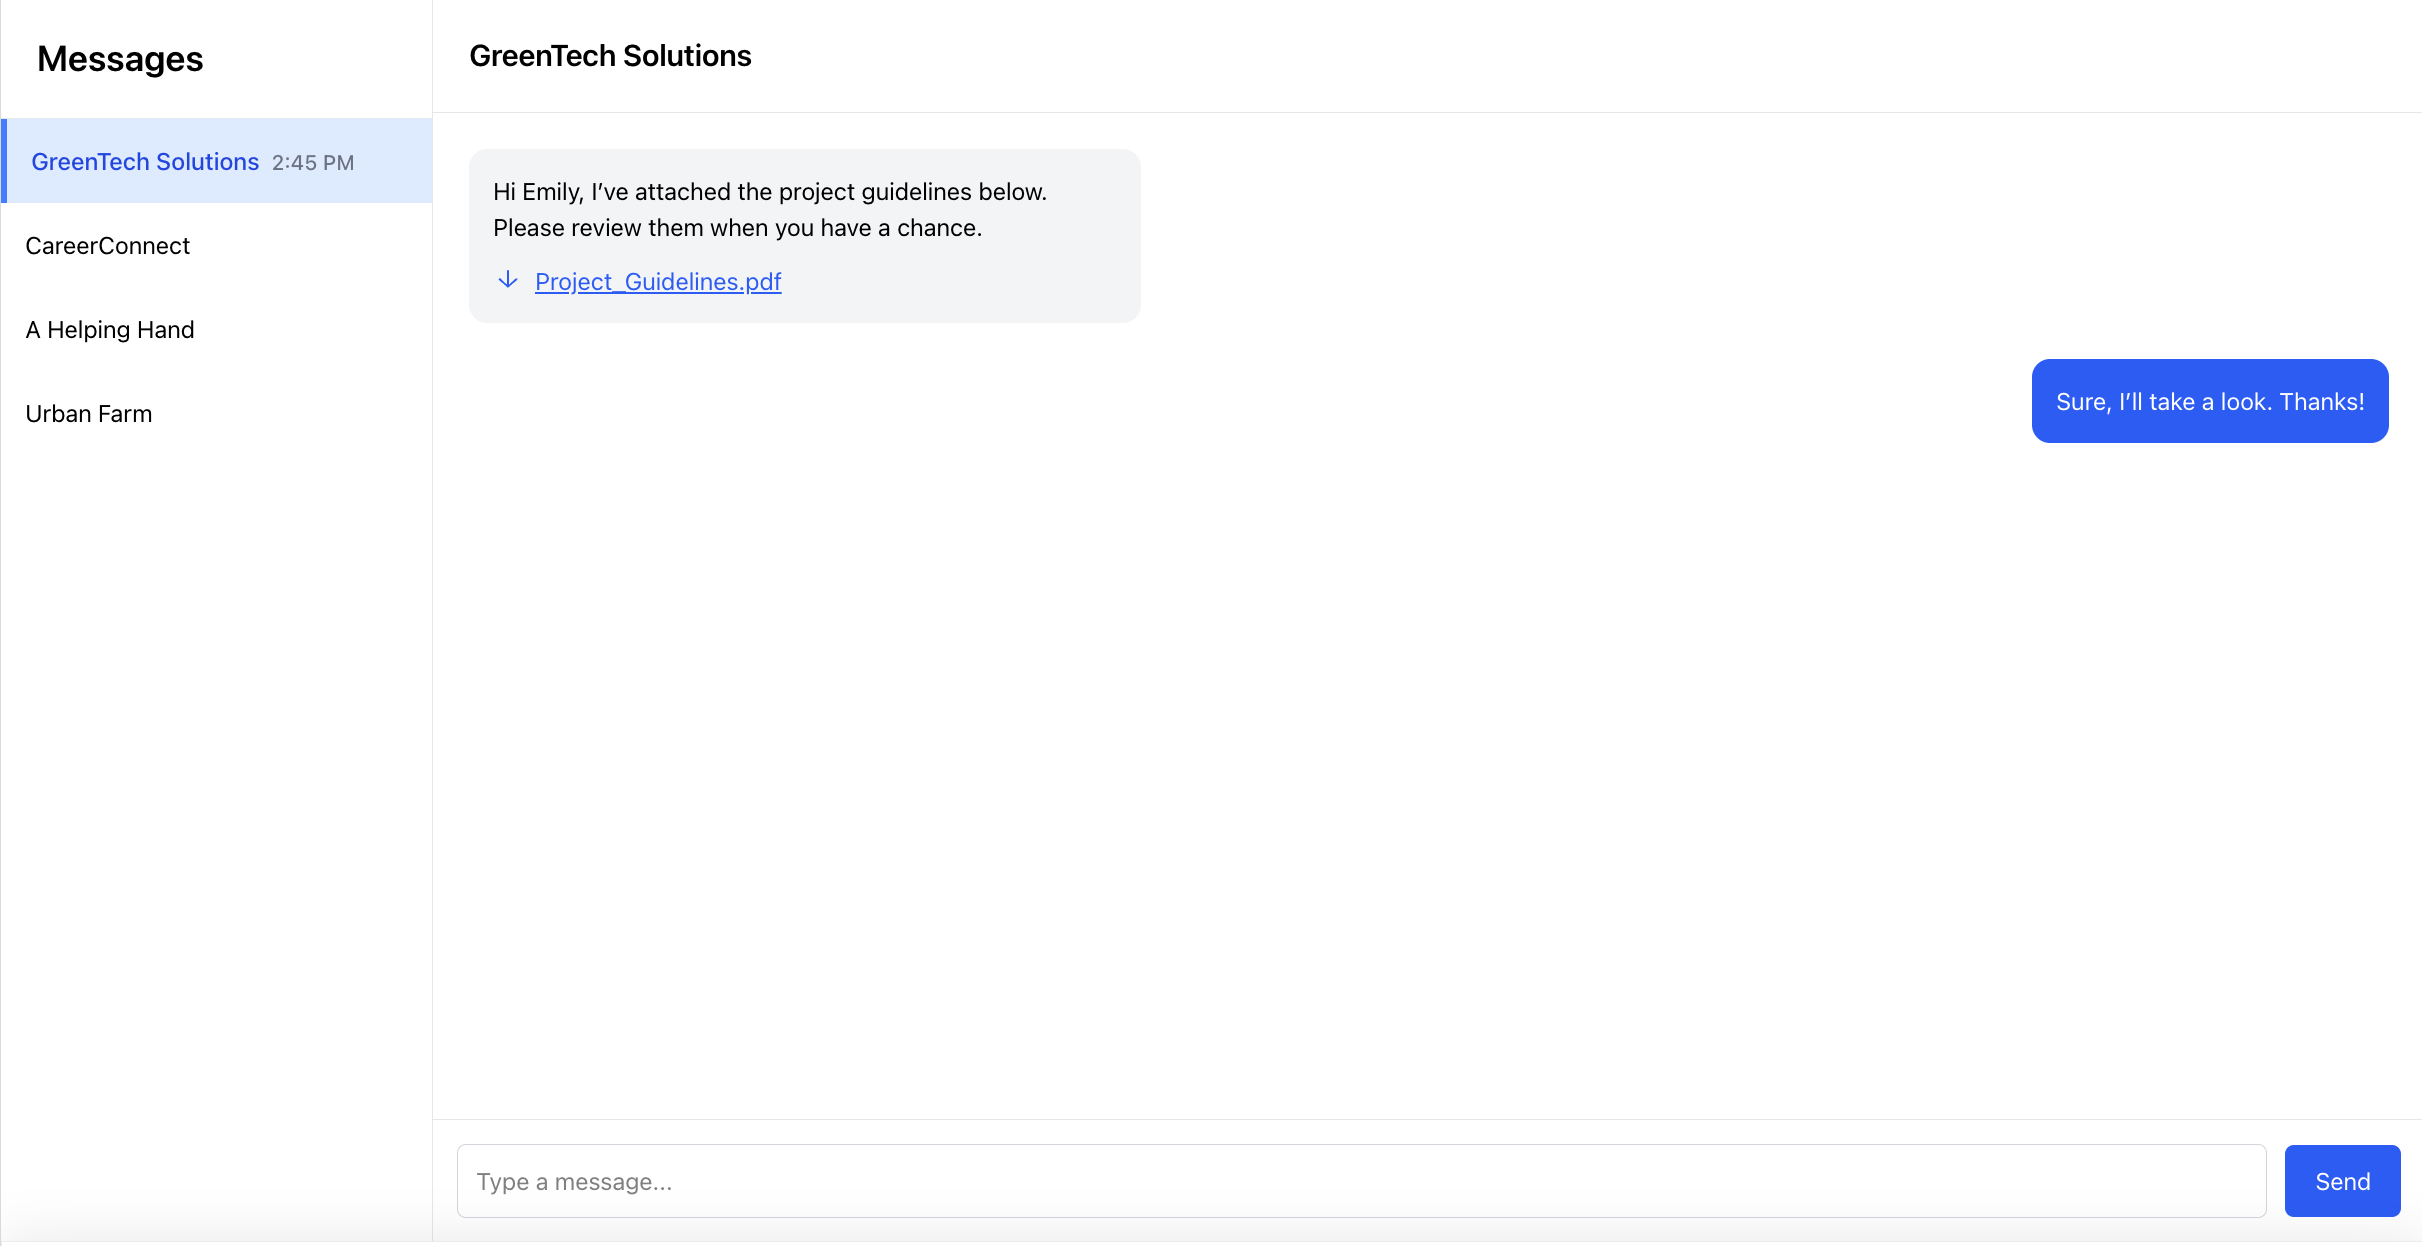
\includegraphics[width=0.85\linewidth]{figures/Messengersystem.png}
  \caption{Messaging workspace (`Messengersystem.png`) used for inclusive support and moderation.}
  \label{fig:chat-system}
\end{figure}

I also introduced a ``mutual aid'' feature where resource-rich partners volunteer surplus capacity (design time, translation, data access) to NGOs with bandwidth gaps. The chat system coordinates offers, logs credits, and routes recognition so inequality does not harden as we scale---a direct response to the gig-work cautionary tales from Lecture~9 \citep{Lecture09}.
